\documentclass[article]{jss}

%% packages
\usepackage{thumbpdf}
\usepackage{amsfonts,amstext,amsmath}
%% need no \usepackage{Sweave.sty}

%% math commands
\newcommand{\R}{\mathbb{R} }
\newcommand{\Var}{\COV}
\newcommand{\V}{\COV}
\newcommand{\z}{\mathbf{z}}
\newcommand{\X}{\mathbf{X}}
\newcommand{\Y}{\mathbf{Y}}
\newcommand{\sX}{\mathcal{X}}
\newcommand{\sY}{\mathcal{Y}}
\newcommand{\T}{\mathbf{T}}
\newcommand{\x}{\mathbf{x}}
\newcommand{\y}{\mathbf{y}}
\renewcommand{\t}{\mathbf{t}}
\renewcommand{\vec}{\text{vec}}

%% code commands
\newcommand{\Rclass}[1]{`\code{#1}'}

%% hyphenation
\hyphenation{Qua-dra-tic}

%% JSS
\author{Torsten Hothorn\\Ludwig-Maximilians-Universit\"at M\"unchen
   \And Kurt Hornik\\Wirtschaftsuniversit\"at Wien
   \AND Mark A.\ van de Wiel\\Vrije Universiteit Amsterdam
   \And Achim Zeileis\\Wirtschaftsuniversit\"at Wien}
\Plainauthor{Torsten Hothorn, Kurt Hornik, Mark A. van de Wiel, Achim Zeileis}

\title{Implementing a Class of Permutation Tests: The \pkg{coin} Package}
\Plaintitle{Implementing a Class of Permutation Tests: The coin Package}
\Shorttitle{\pkg{coin}: Implementing a Class of Permutation Tests}

\Abstract{
  The \proglang{R} package \pkg{coin} implements a unified approach to
  permutation tests providing a huge class of independence tests  
  for nominal, ordered, numeric, and censored data as well as
  multivariate data at mixed scales. Based on a rich and flexible
  conceptual framework that embeds different permutation test procedures into a common
  theory, a computational framework is established in \pkg{coin} that
  likewise embeds the corresponding \proglang{R} functionality in a common
  \proglang{S}4 class structure with associated generic functions.
  As a consequence, the computational tools in \pkg{coin} inherit
  the flexibility of the underlying theory and conditional inference
  functions for important special cases can be set up easily. 
  Conditional versions of classical tests---such 
  as tests for location and scale problems in
  two or more samples, independence in two- or three-way contingency tables,
  or association problems for censored, ordered categorical or multivariate data---can 
  easily be implemented as special cases using this computational 
  toolbox by choosing appropriate transformations of the observations.
  The paper gives a detailed exposition of both the internal structure
  of the package and the provided user interfaces along with examples on how
  to extend the implemented functionality.
}

\Keywords{conditional inference, exact distribution, conditional Monte Carlo, categorical data analysis, \proglang{R}}
\Plainkeywords{conditional inference, exact distribution, conditional Monte Carlo, categorical data analysis, R}

%% \Volume{13}
%% \Issue{9}
%% \Month{September}
%% \Year{2004}
%% \Submitdate{2004-09-29}
%% \Acceptdate{2004-09-29}

\Address{
  Torsten Hothorn\\
  Institut f\"ur Statistik\\
  Ludwig-Maximilians-Universit\"at M\"unchen\\
  Ludwigstra{\ss}e 33\\
  DE-80539 M\"unchen, Germany \\
  E-mail: \email{Torsten.Hothorn@R-project.org}\\
  URL: \url{http://www.stat.uni-muenchen.de/~hothorn/}\\

  Kurt Hornik, Achim Zeileis\\
  Department of Statistics and Mathematics\\
  Wirtschaftsuniversit\"at Wien\\
  Augasse 2--6\\
  AT-1090 Wien, Austria\\
  E-mail: \email{Kurt.Hornik@R-project.org}, \email{Achim.Zeileis@R-project.org}\\

  Mark A.\ van de Wiel\\
  Department of Mathematics\\
  Vrije Universiteit Amsterdam\\
  De Boelelaan 1081a\\
  NL-1081 HV Amsterdam, The Netherlands\\
  E-mail: \email{mark.vdwiel@vumc.nl}
}





\begin{document}

\section{Introduction}

Conditioning on all admissible permutations of the data for testing 
independence hypotheses is a very old, yet very powerful and popular, 
idea \citep{fisher1935,Ernst2004}. Conditional
inference procedures, or simply \textit{permutation} or \textit{re-randomization}
tests, are implemented in 
many different statistical computing environments.
These implementations, for example 
\code{wilcox.test()} for the Wilcoxon-Mann-Whitney test or
\code{mantelhaen.test()} for the Cochran-Mantel-Haenszel $\chi^2$ test in \proglang{R} \citep{rcore2007} 
or the tools implemented in \pkg{StatXact} \citep{StatXact6}, 
\pkg{LogXact} \citep{LogXact8}, or \proglang{Stata} \citep{Stata}---see \cite{Oster2002,Oster2003} 
for an overview---all follow the classical classification scheme of inference procedures and
offer procedures for location problems, scale problems, correlation, 
or nominal and ordered categorical data. 
Thus, each test procedure is 
implemented separately, maybe with the exception of conditional 
versions of linear rank statistics \citep{theory-of-:-1999} in \texttt{NPAR1WAY}
as available in \proglang{SAS} \citep{SAS}.

Theoretical insights by \cite{StrasserWeber1999} open up the way
to a unified treatment of a huge class of permutation
tests. The \pkg{coin} package for \underline{co}nditional \underline{in}ference
is the computational counterpart to this theoretical framework,
implemented in the \proglang{R} system for statistical computing \citep{rcore2007}.
\cite{Hothorn:2006:AmStat} introduce the package and illustrate the
transition from theory to practice. Here, we focus on the design principles upon which the
\pkg{coin} implementation is based as well as on the more technical issues
that need to be addressed in the implementation of such conceptual
tools.
Within package \pkg{coin}, formal \proglang{S}4 classes describe the data model 
and the conditional test procedures, 
consisting of multivariate linear statistics, univariate test statistics 
and a reference distribution. Thus, one can work with objects representing 
the theoretical entities nearly in the same way as one would work
with mathematical symbols. Generic functions for obtaining
statistics, conditional expectation and covariance matrices as well as 
$p$~value, distribution, density and quantile functions for the reference
distribution help to extract information from these objects.
The infrastructure is conveniently interfaced in the function \code{independence_test()},
thus providing the computational counterpart of the theoretical framework of
\cite{StrasserWeber1999}.

Here, we start out with an illustrative application of \code{independence_test()}
to a small 2-sample problem (see Table~\ref{rotarod}) and then continue to
introduce the underlying computational building blocks using the same data set.
The data was used previously by \cite{Bergmann:2000} as a challenging example
in a comparison of test statistics and $p$~values of the Wilcoxon-Mann-Whitney
rank sum test as reported by eleven statistical packages. 
More specifically, $n = 24$ rats received a fixed oral dose of a centrally 
acting muscle relaxant as active treatment or a saline solvent as control. The animals were 
placed on a rotating cylinder and the length of time each rat remained on the cylinder was
measured, up to a maximum of $300$ seconds. The rats were randomly assigned to the control 
and treatment groups, thus a re-randomization test as implemented 
in \code{independence_test()} is the appropriate way to investigate
if the response is independent of the group assignment. The data are particularly
challenging because of the many ties in the (censored) response ($19$
observations take the maximal value $300$) and the quasi-complete separation (smaller values of time
are only observed in the treatment group). Conceptually, this makes computation of the
two-sided exact $p$~value for any 2-sample contrast very simple:
$p = 2 \cdot {19 \choose 12} / {24 \choose 12} =
0.03727$. However,
in software, this often makes computations of the exact $p$~value more difficult
because several simple algorithms fail.

\begin{table}[t]
\begin{center}
\begin{tabular}{|r|rrrrrrrrrrrr|}
\hline
\code{group} & \multicolumn{12}{|l|}{\code{time}} \\ \hline
control & 300 & 300 & 300 & 300 & 300 & 300 & 300 & 300 & 300 & 300 & 300 & 300 \\
treatment & 18 & 22 & 75 & 163 & 271 & 300 & 300 & 300 & 300 & 300 & 300 & 300 \\
\hline
\end{tabular}
\caption{The \code{rotarod} data: length of \code{time} on rotating cylinder by
\code{group}.  \label{rotarod}} 
\end{center}
\end{table}

Utilizing \pkg{coin}, the hypothesis of independence of length of time and group assignment can
be specified by a formula which, together with a data frame \code{rotarod}, 
serve as arguments to \code{independence_test}: 
\begin{Schunk}
\begin{Sinput}
R> library("coin")
R> data("rotarod", package = "coin")
R> independence_test(time ~ group, data = rotarod,
+    ytrafo = rank, distribution = exact())
\end{Sinput}
\begin{Soutput}
	Exact General Independence Test

data:  time by group (control, treatment) 
Z = 2.4389, p-value = 0.03727
alternative hypothesis: two.sided 
\end{Soutput}
\end{Schunk}
Here, the conditional Wilcoxon-Mann-Whitney test was performed
via a rank transformation of the response, employing the exact distribution for
obtaining the $p$~value (yielding the correct result outlined above).
Users of \proglang{R} can easily interpret this output since
it is represented in the same format as classical tests in the basic
\pkg{stats} package. Based on the $p$~value derived from
the exact conditional distribution of the test statistic \code{Z},
the independence of group assignment and time on the cylinder can be rejected.

Although the above piece of code looks embarrassingly simple, the
underlying computations are much more sophisticated than visible at
first sight: The data are pre-processed along with their
transformations, deviations from independence are captured by a
(possibly multivariate) linear statistic, standardized by conditional
expectation and variance, and aggregated to a final test
statistic. Subsequently, the requested reference distribution is
computed, from which a $p$~value is derived, and everything is wrapped
into an object that can be conveniently printed or queried for more
detailed information. After briefly reviewing the underlying theory from
\cite{StrasserWeber1999} in Section~\ref{sec:theory}, we introduce
formal \proglang{S}4 classes and methods capturing all the outlined
steps in Section~\ref{sec:class}. Section~\ref{sec:ui} provides further
information about high-level user interfaces and extensibility, and
Section~\ref{sec:practice} further illustrates how to employ the
software in practice using a categorical data example.
Section~\ref{sec:oddsandends} concludes the paper with a short
discussion, some more details about the underlying theory can be found
in an appendix.

\section{Permutation tests in a nutshell} \label{sec:theory}

In the following we give a brief overview of the general theory for permutation tests
as developed by \cite{StrasserWeber1999} and implemented by \cite{Hothorn:2006:AmStat}.

The task is to test the independence of two variables $\Y$ and $\X$ 
from sample spaces $\mathcal{Y}$ and $\mathcal{X}$ which may
be measured at arbitrary scales and may be multivariate as well.
In addition, $b \in \{1, \dots, k\}$, a factor measured at $k$ levels, indicates a certain block
structure of the observations: for example study centers in a
multi-center randomized clinical trial where only a re-randomization of observations within blocks
is admissible. 
We are interested in testing the null hypothesis
\begin{eqnarray*}
  H_0: D(\Y | \X, b) = D(\Y | b)
\end{eqnarray*}
of conditional independence of $\Y$ and $\X$ within blocks~$b$ against
arbitrary alternatives, for example shift or scale alternatives, linear trends,
association in contingency tables etc.
\cite{StrasserWeber1999} suggest deriving 
scalar test statistics for testing $H_0$ from multivariate linear statistics
of the form 
\begin{eqnarray} \label{linstat}
\T =  \sum_{j = 1}^k \T_j \in \R^{pq}
\end{eqnarray}
where the linear statistic for each block is given by
\begin{eqnarray*}
\T_j = \vec\left(\sum_{i = 1}^n I(b_i = j) w_i g(\X_i) h(\Y_i)^\top\right)
\in \R^{pq}.
\end{eqnarray*}
The function $I(\cdot)$ is the indicator function and $\vec$
denotes the vec operator (which stacks the columns of a matrix).  
Here, $g: \mathcal{X} \rightarrow \R^{p \times 1}$ is a transformation of
the $\X$ measurements and $h: \mathcal{Y} \rightarrow
\R^{q \times 1}$ is a transformation of the $\Y$ values. The function $h(\Y_i)
= h(\Y_i, (\Y_1, \dots, \Y_n))$ is also called \emph{influence function} and
may depend on the full vector of responses
$(\Y_1, \dots, \Y_n)$, however only 
in a permutation symmetric way, i.e., the value of the
function must not depend on the order in which $\Y_1, \dots, \Y_n$ appear.
The case weights $w_i$ are assumed to be integer-valued, indicating
that $w_i$ observations with realizations $\Y_i$, $\X_i$ and $b_i$
are available, with default $w_i \equiv 1$.

The distribution of $\T$  depends on the joint
distribution of $\Y$ and $\X$, which is unknown under almost all practical
circumstances. At least under the null hypothesis one can dispose of this
dependency by fixing $\X_1, \dots, \X_n$ and conditioning on all possible
permutations of the responses $\Y_1, \dots, \Y_n$ within block $j, j = 1, \dots, k$. 
The conditional expectation $\mu \in \R^{pq}$ and covariance 
$\Sigma \in \R^{pq \times pq}$ 
of $\T$ under $H_0$ given
all permutations $\sigma \in S$ of the responses are derived by
\cite{StrasserWeber1999} and are given in Appendix~\ref{app}.
Having the conditional expectation and covariance at hand we are able to
standardize an observed linear statistic $\t \in \R^{pq}$ (of the form
given in Equation~\ref{linstat}) and aggregate it to some univariate test
statistic $c = c(\t, \mu,\Sigma)$. Various choices for $c(\t, \mu,\Sigma)$
are conceivable, e.g., a quadratic form or a maximum type statistic
(see Section~\ref{sec:class}). 
In the latter case, a natural first step
is to standardize each of the $pq$ statistics in $\t$ by its expectation and
standard deviation:
\begin{eqnarray} \label{standstat}
\z = \text{diag}(\Sigma)^{-1/2} (\mathbf{t} - \mu).
\end{eqnarray}

In the following, we describe a class structure for representing these
theoretical objects along with possible choices of test statistics $c$
and computations or approximations of the associated reference
distributions.


\section{A class structure for permutation tests} \label{sec:class}

In this section, the theory of permutation tests, as briefly outlined in the previous
section, is captured in a set of \proglang{S}4 classes and methods: In
Section~\ref{sec:data}, we suggest objects representing the data and the independence
problem, for which a test statistic is computed subsequently.
Objects for the associated reference distribution are constructed in Section~\ref{sec:distr}.
Finally, in Section~\ref{sec:testobj}, everything is combined in a single object
for the whole testing procedure.

\subsection{Data, independence problems and test statistics} \label{sec:data}

\subsubsection{Data structure}

We are provided with $n$ observations 
$(\Y_i, \X_i, b_i, w_i), i = 1, \dots, n.$
In addition to variables $\X$, $\Y$, and $b$, it is convenient (for
example to efficiently represent large contingency tables)
to include case weights $w_i$, defaulting to $w_i \equiv 1$.
This data structure is represented by class \Rclass{IndependenceProblem}:
\begin{center}
\begin{tabular}{ll}
\multicolumn{2}{l}{Class \Rclass{IndependenceProblem}} \\
 & \\
Slot & Class \\ \hline 
\code{x} & \Rclass{data.frame} \\
\code{y} & \Rclass{data.frame} \\
\code{block} & \Rclass{factor} \\
\code{weights} & \Rclass{numeric} \\
\hline
\end{tabular}
\end{center}Note that objects of this class implicitly define the null distribution
$H_0$ and all admissible permutations of observations within blocks.

For our illustrating rotating rats example, we specify the hypothesis
of independence of variables \code{time} and \code{group} by initializing a new
independence problem with the corresponding observations:
\begin{Schunk}
\begin{Sinput}
R> ip <- new("IndependenceProblem",
+    y = rotarod["time"], x = rotarod["group"])
\end{Sinput}
\end{Schunk}

\subsubsection{Independence problems and linear statistics}

The transformation functions $g$ and $h$ as well as the transformed observations
$g(\X_i)$ and $h(\Y_i), i = 1, \dots, n$, are added to the data structure
by extending class \Rclass{IndependenceProblem}:
\begin{center}
\begin{tabular}{ll}
\multicolumn{2}{l}{Class \Rclass{IndependenceTestProblem}} \\
\multicolumn{2}{l}{Contains \Rclass{IndependenceProblem}} \\
 & \\
Slot & Class \\ \hline 
\code{xtrans} & \Rclass{matrix} \\
\code{ytrans} & \Rclass{matrix} \\
\code{xtrafo} & \Rclass{function} \\
\code{ytrafo} & \Rclass{function} \\
\hline
\end{tabular}
\end{center}The \code{ytrafo} and \code{xtrafo} slots correspond to the transformations
$h$ and $g$, respectively. The $i$th row of the 
$n \times q$ matrix \code{ytrans} corresponds to $h(\Y_i)$. Similarly, 
the rows of \code{xtrans} ($n \times p$) correspond to $g(\X_i)$. 
Note that, in addition to the data, hypothesis and permutation scheme, the
test statistic $\T$ is defined by objects of class \Rclass{IndependenceTestProblem}
as well.

In the simplest case of both $\X$ and $\Y$ being univariate 
factors at $p$ and $q$ levels, $g$ and $h$ are 
the corresponding dummy codings and the linear statistic $\T$ is the
(vectorized) $p \times q$ contingency table of $\X$ and $\Y$. In the rats example,
the default dummy coding for factor \code{group} is employed and a rank
transformation (via \code{rank()}) is applied to \code{time}.
\begin{Schunk}
\begin{Sinput}
R> itp <- new("IndependenceTestProblem", ip, ytrafo = rank)
\end{Sinput}
\end{Schunk}

The linear statistic $\T$, its conditional expectation $\mu$ and covariance $\Sigma$
are stored in objects of class \Rclass{IndependenceLinearStatistic}:
\begin{center}
\begin{tabular}{ll}
\multicolumn{2}{l}{Class \Rclass{IndependenceLinearStatistic}} \\
\multicolumn{2}{l}{Contains \Rclass{IndependenceTestProblem}} \\
 & \\
Slot & Class \\ \hline 
\code{linearstatistic} & \Rclass{numeric} \\
\code{expectation} & \Rclass{numeric} \\
\code{covariance} & \Rclass{VarCovar} \\
\hline
\end{tabular}
\end{center}Class \Rclass{VarCovar} represents either a complete covariance matrix 
or its diagonal elements only. By default, only the conditional variances
are stored, the whole covariance matrix can be computed as needed (see below).
In the rotating rats example, such an object is easily created via

\begin{Schunk}
\begin{Sinput}
R> ils <- new("IndependenceLinearStatistic", itp)
\end{Sinput}
\end{Schunk}

Using methods for suitable generic functions (see Table~\ref{tab:generics}),
the linear statistic for the rotating rats can be extracted via
\begin{Schunk}
\begin{Sinput}
R> statistic(ils, "linear")
\end{Sinput}
\begin{Soutput}
control 180
\end{Soutput}
\end{Schunk}
This is simply the sum of the average ranks in the control group, i.e., $180 = 12 \cdot 15$
because all 12 observations have the maximal average rank 15. Additionally, the associated
conditional mean and variance under $H_0$ can be computed via:
\begin{Schunk}
\begin{Sinput}
R> expectation(ils)
\end{Sinput}
\begin{Soutput}
control 
    150 
\end{Soutput}
\begin{Sinput}
R> variance(ils)
\end{Sinput}
\begin{Soutput}
 control 
151.3043 
\end{Soutput}
\end{Schunk}
based upon which we can now set up a test statistic. 


\subsubsection{Test statistics} \label{sec:teststat}

\begin{table}[tb]
\begin{center}
\begin{tabular}{lp{9.5cm}}
\hline
Function & Description \\ \hline
\code{statistic(object, type)} & Extraction of the linear statistic $\t$ (\code{type = "linear"}), 
		     the standardized statistic $\z$ (\code{type = "standardized"})
  		     or the final test statistic $c$ (\code{type = "test"}, only for
		     objects inheriting from \Rclass{IndependenceTestStatistic}). \\
\code{expectation(object)} & Extraction of the conditional expectation~$\mu$. \\
\code{covariance(object)} & Extraction of the complete conditional covariance
  matrix~$\Sigma$. \\
\code{variance(object)} & Extraction of the diagonal elements of the conditional covariance matrix
                          $\text{diag}(\Sigma)$. \\ \hline
\end{tabular}
\caption{\label{tab:generics} List of generic functions with
  methods for classes inheriting from \Rclass{IndependenceLinearStatistic}.}
\end{center}
\end{table}


The specification of the inference procedure is completed by the definition
of a univariate test statistic $c$
which is represented by a virtual class \Rclass{IndependenceTestStatistic}
\begin{center}
\begin{tabular}{ll}
\multicolumn{2}{l}{Class \Rclass{IndependenceTestStatistic}} \\
\multicolumn{2}{l}{Contains \Rclass{IndependenceLinearStatistic}} \\
 & \\
Slot & Class \\ \hline 
\code{teststatistic} & \Rclass{numeric} \\
\code{standardizedlinearstatistic} & \Rclass{numeric} \\
\hline
\end{tabular}
\end{center}The slot \code{standardizedlinearstatistic}
contains $\z$, the (possibly multivariate) linear statistic standardized by its 
conditional expectation and variance (Equation~\ref{standstat}). 
Slot \code{teststatistic} is for storing univariate test statistics $c$?
\begin{Schunk}
\begin{Sinput}
R> its <- new("IndependenceTestStatistic", ils)
\end{Sinput}
\end{Schunk}
Methods for all generics listed in Table~\ref{tab:generics}
are also available for objects of this class.

The slot \code{teststatistic} has not yet been filled in the
\Rclass{IndependenceTestStatistic} object. \pkg{coin} implements
three sub-classes with associated univariate test statistics for this:
scalar test statistics $c_\text{scalar}$, maximum-type statistics $c_\text{max}$ and quadratic
forms $c_\text{quad}$.
In case of univariate linear statistics $\t$, i.e., for $pq = 1$, a natural test statistic $c$
is simply the standardized linear statistic
\begin{eqnarray*}
c_\text{scalar}(\t, \mu, \Sigma) = 
\frac{\t - \mu}{\sqrt{\Sigma}} = \z.
\end{eqnarray*} 
A special class is available for this
\begin{center}
\begin{tabular}{ll}
\multicolumn{2}{l}{Class \Rclass{ScalarIndependenceTestStatistic}} \\
\multicolumn{2}{l}{Contains \Rclass{IndependenceTestStatistic}} \\
 & \\
Slot & Class \\ \hline 
\code{alternative} & \Rclass{character} \\
\hline
\end{tabular}
\end{center}that also defines a character vector specifying the alternative to 
test against (\code{"two.sided"}, \code{"greater"} and \code{"less"}).
Thus, the construction  of a scalar test statistic corresponds
to the construction of a suitable object via
\begin{Schunk}
\begin{Sinput}
R> sits <- new("ScalarIndependenceTestStatistic", its,
+    alternative = "two.sided")
R> statistic(sits, "standardized")
\end{Sinput}
\begin{Soutput}
control 2.438909
\end{Soutput}
\end{Schunk}
which yields the standardized Wilcoxon-Mann-Whitney statistic reported
in the introductory example.
In the multivariate case ($pq > 1$), a natural extension is to employ a
maximum-type statistic of the form
\begin{displaymath}
  c_\text{max}(\mathbf{t}, \mu, \Sigma)  = 
  \begin{cases}
    \max \left| \z \right| & \text{(``two-sided'')}, \\
    \min \left( \z \right) & \text{(``less'')}, \\
    \max \left( \z \right) & \text{(``greater'')},
  \end{cases}
\end{displaymath}
where the definition reflects the associated alternative with name given
in quotes.  Again a special class
\Rclass{MaxTypeIndependenceTestStatistic} is available for this:
\begin{center}
\begin{tabular}{ll}
\multicolumn{2}{l}{Class \Rclass{MaxTypeIndependenceTestStatistic}} \\
\multicolumn{2}{l}{Contains \Rclass{IndependenceTestStatistic}} \\
 & \\
Slot & Class \\ \hline 
\code{alternative} & \Rclass{character} \\
\hline
\end{tabular}
\end{center}

Alternatively, a quadratic form $c_\text{quad}(\mathbf{t}, \mu, \Sigma)  =
(\mathbf{t} - \mu)^\top \Sigma^+ (\mathbf{t} - \mu)$ can be used as test statistic. It
is computationally more expensive because the Moore-Penrose 
inverse $\Sigma^+$ of $\Sigma$ is involved. Such statistics are represented
by objects of class \Rclass{QuadTypeIndependenceTestStatistic} defining slots 
for $\Sigma^+$ and its rank (degrees of freedom):
\begin{center}
\begin{tabular}{ll}
\multicolumn{2}{l}{Class \Rclass{QuadTypeIndependenceTestStatistic}} \\
\multicolumn{2}{l}{Contains \Rclass{IndependenceTestStatistic}} \\
 & \\
Slot & Class \\ \hline 
\code{covarianceplus} & \Rclass{matrix} \\
\code{df} & \Rclass{numeric} \\
\hline
\end{tabular}
\end{center}A slot \code{alternative} is not needed because, by construction,
quadratic forms cannot be applied to one-sided hypotheses.

\subsection{Representation of conditional null distributions} \label{sec:distr}

The conditional distribution (or an approximation thereof)
and thus the $p$~value corresponding to the statistic $c(\mathbf{t}, \mu, \Sigma)$ can be
computed in several different ways. For some special forms of the
linear statistic, the exact distribution of the test statistic is tractable.
For 2-sample problems, the shift algorithm by \cite{axact-dist:1986,exakte-ver:1987} 
and the split-up algorithm by 
\cite{vdWiel2001} are implemented as part of the package.

Conditional Monte-Carlo procedures can always be used to approximate the exact
distribution. In this case, within each block, a sufficiently large number of
random samples from all admissible permutations of the observations is drawn. The 
test statistic is computed for the permuted $\X$ values and the 
distribution of these test statistics is an approximation to the 
conditional reference distribution. When $p$~values are computed,
confidence intervals are available from the binomial distribution.

\citet[Theorem 2.3]{StrasserWeber1999} showed that the   
conditional distribution of linear statistics $\T$ with conditional    
expectation $\mu$ and covariance $\Sigma$ tends to a multivariate normal
distribution with parameters $\mu$ and $\Sigma$ as $\sum_{i = 1}^n I(b_i = j)w_i \rightarrow \infty$ for all $j = 1, \dots, k$. 
Thus, the asymptotic conditional distribution of the standardized linear statistic $\z$ 
is normal and therefore, $p$~values for scalar or maximum-type univariate statistics
can be computed directly in the univariate case ($pq = 1$) 
or approximated by numerical algorithms
\citep{numerical-:1992} as implemented
in package \pkg{mvtnorm} \citep{PKG:mvtnorm}
in the multivariate setting. For quadratic forms
$c_\text{quad}$ which follow a $\chi^2$ distribution with degrees of freedom 
given by the rank of $\Sigma$ \citep[see][Chapter 29]{johnsonkotz1970},
asymptotic probabilities can be computed straightforwardly.

A null distribution is represented by either a distribution (and $p$~value) function
only
\begin{center}
\begin{tabular}{ll}
\multicolumn{2}{l}{Class \Rclass{PValue}} \\
 & \\
Slot & Class \\ \hline 
\code{pvalue} & \Rclass{function} \\
\code{p} & \Rclass{function} \\
\code{name} & \Rclass{character} \\
\hline
\end{tabular}
\end{center}or, where possible, is augmented by its density and quantile functions:
\begin{center}
\begin{tabular}{ll}
\multicolumn{2}{l}{Class \Rclass{NullDistribution}} \\
\multicolumn{2}{l}{Contains \Rclass{PValue}} \\
 & \\
Slot & Class \\ \hline 
\code{q} & \Rclass{function} \\
\code{d} & \Rclass{function} \\
\code{support} & \Rclass{function} \\
\code{parameters} & \Rclass{list} \\
\hline
\end{tabular}
\end{center}Currently, there are three classes extending \Rclass{NullDistribution} (without 
defining additional slots at the moment): \Rclass{ExactNullDistribution},
\Rclass{ApproxNullDistribution}, and \Rclass{AsymptNullDistribution}.
All of them can be queried for probabilities, quantiles, etc., using
suitable methods (see Table~\ref{tab:dists} for an overview).
New methods for computing or approximating the conditional distribution
can be integrated into the framework via suitable
inheritance from \Rclass{PValue} (an example is given in Section~\ref{sec:ui}).

\begin{table}[tb]
\begin{center}
\begin{tabular}{lp{9.5cm}}
\hline
Class & Description \\
\hline
\Rclass{ExactNullDistribution} & Exact conditional null distribution (e.g.,
  computed via the shift algorithm). \\
\Rclass{ApproxNullDistribution} & Approximation of the exact conditional 
  distribution using conditional Monte-Carlo procedures. \\
\Rclass{AsymptNullDistribution} & Asymptotic conditional 
  distribution (via multivariate normal or $\chi^2$ distribution). \\
\hline
Method & Description \\
\hline
\code{pvalue(object)} & Computation of the $p$~value (plus a confidence interval if
  Monte-Carlo procedures have been used) based on an observed test statistic $c$ and its
  conditional null distribution. \\
\code{pperm(object, q)} & Evaluation of the cumulative distribution function for quantile $q$.\\
\code{dperm(object, x)} & Evaluation of the probability density function at $x$. \\
\code{qperm(object, p)} & Evaluation of the quantile function for probability $p$.\\
\code{support(object)}  & Extraction of the support of the null distribution.\\
\hline
\end{tabular}
\caption{\label{tab:dists} Classes and methods for conditional null distributions.}
\end{center}
\end{table}
The \code{support} function returns the support of a discrete distribution or
an interval containing $99.999\%$ of the probability mass.



Using these tools, the exact $p$~value for the independence test on the rotating rats
along with the complete exact reference distribution (allowing
for the computation of quantiles, for example) can be derived via
\begin{Schunk}
\begin{Sinput}
R> end <- ExactNullDistribution(sits)
R> pvalue(end, statistic(sits))
\end{Sinput}
\begin{Soutput}
[1] 0.03726708
\end{Soutput}
\begin{Sinput}
R> qperm(end, 0.95)
\end{Sinput}
\begin{Soutput}
[1] 1.544642
\end{Soutput}
\end{Schunk}

For maximum-type statistics $c_\text{max}$, single-step and step-down
multiplicity adjusted $p$~values based on the limiting distribution and
conditional Monte-Carlo methods \citep[see][]{WestfallYoung1993} are
available as well.


\subsection{Objects for conditional tests} \label{sec:testobj}

A conditional test is represented by a test statistic of class \Rclass{IndependenceTestStatistic}
and its conditional null distribution inheriting from class \Rclass{PValue}. 
In addition, a character string giving the name of the test procedure is defined 
in class \Rclass{IndependenceTest}:
\begin{center}
\begin{tabular}{ll}
\multicolumn{2}{l}{Class \Rclass{IndependenceTest}} \\
 & \\
Slot & Class \\ \hline 
\code{distribution} & \Rclass{PValue} \\
\code{statistic} & \Rclass{IndependenceTestStatistic} \\
\code{estimates} & \Rclass{list} \\
\code{method} & \Rclass{character} \\
\hline
\end{tabular}
\end{center}Remember that objects of class \Rclass{IndependenceTestStatistic} 
represent the data, hypothesis, linear statistic and test statistic along with
conditional expectation and covariance matrix.
The \code{estimates} slot
may contain parameter estimates where available, for example 
an estimate and corresponding confidence interval for a shift parameter
derived from a conditional Wilcoxon-Mann-Whitney test.

A complete description of the conditional independence test for the rotating
rats data is given by an object of class \Rclass{IndependenceTest} which
is conveniently represented by the corresponding \code{show()} method:
\begin{Schunk}
\begin{Sinput}
R> new("IndependenceTest", statistic = sits, distribution = end)
\end{Sinput}
\begin{Soutput}
	Exact General Independence Test

data:  time by group (control, treatment) 
c = 2.4389, p-value = 0.03727
\end{Soutput}
\end{Schunk}
Of course, the methods previously defined in this section
(see Tables~\ref{tab:generics} and \ref{tab:dists}) are defined for
objects of class \Rclass{IndependenceTest} as well. Thus, all theoretical entities
introduced in Section~\ref{sec:theory} are now captured in a single
object of class \Rclass{IndependenceTest} and all methods for extracting 
information from it are readily available.


\section{Interfaces to permutation inference} \label{sec:ui}

In Section~\ref{sec:class}, all the necessary computational building blocks are
introduced for implementing the general class of permutation tests outlined
in Section~\ref{sec:theory}. However, one rarely needs to exploit the full
flexibility of each component of the framework. More often, one wants to employ
sensible defaults for most (if not all) steps in the analysis but preserving
the possibility to extend a few steps based on user-supplied methods.
For this purpose, \pkg{coin} provides the function \code{independence_test()}
as the main user interface for performing independence tests. Many of its arguments
have flexible defaults or can be specified by a simple character string while
still allowing to plug in much more complex user-defined objects, e.g., for 
data preparation, computation of the null distribution, or transformation functions.

\subsection{A convenient user interface}

Via the generic function \code{independence_test()}, all steps described
in Section~\ref{sec:class} can be carried out using a single command.
The main workhorse behind it is the method for objects of class
\Rclass{IndependenceProblem}:
\begin{Sinput}
independence_test(object, 
  teststat = c("max", "quad", "scalar"),
  distribution = c("asymptotic", "approximate", "exact"),
  alternative = c("two.sided", "less", "greater"),
  xtrafo = trafo, ytrafo = trafo, scores = NULL, 
  check = NULL, ...)
\end{Sinput}
Thus, \code{object} describes the data and the null hypothesis. Arguments
\code{xtrafo} and \code{ytrafo} refer to the transformations $g$ and $h$: Both are
by default set to function \code{trafo()} which chooses suitable transformations
based on the scale of the considered variables (see below). 
The three types of univariate test statistics discussed above are hard-coded and can be specified by 
a simple string. Similarly, the reference distribution and the alternative hypothesis
can be supplied as strings. In addition to these simple specifications, more flexible
specifications for the data (\code{object}), the transformations (\code{xtrafo}, \code{ytrafo}),
and the distribution are available, as discussed in the following. The \code{scores}
argument takes a named list of numeric vectors to be used as scores for ordered
factors. Validity checks for objects of class \Rclass{IndependenceProblem} specified
to argument \code{check} can be used to test for certain aspects of the data, e.g.,
when one has to make sure that two independent samples are present.

\subsection{Data specification}

The standard way of specifying relationships between variables in \proglang{R}
are formulas in combination with a data frame. Hence, a \Rclass{formula} method
for \code{independence_test()} is provided that interprets the left hand side
variables of a formula as $\Y$ variables (univariate or possibly multivariate),
the right hand side as $\X$ variables (univariate or multivariate as well).
An optional blocking factor can specified after a vertical bar, e.g.,
\begin{Sinput}
y1 + y2 ~ x1 + x2 | block
\end{Sinput}
This specifies an independence problem between two $\Y$ variables and two $\X$ variables (in case
all variables are numeric the linear statistic is 4-dimensional with 
$p = 2$ and $q = 2$) for each level in \code{block}. As usual, \code{data}, \code{weights}
and \code{subset} arguments can be specified as well. Based on all these
arguments the \Rclass{IndependenceProblem} is built and simply passed on
to the \code{independence_test()} method described above.

For (simple) categorical data, there is yet another way of specifying the 
independence problem, namely via the \Rclass{table} method of
\code{independence_test()}. Its first argument is allowed to be a 2- or 3-dimensional
table: The first two margins are interpreted as univariate categorical 
$\X$ and $\Y$ variables and the optional third margin is taken to be the
blocking factor. Again, an \Rclass{IndependenceProblem} object is derived
from this and passed on to the associated method.


\subsection{Null distributions}

In the simplest case, the \code{distribution} argument of the \code{independence_test()}
methods can be specified by a simple character string. However, this
is not flexible enough in some situations and hence it is also possible to
supply a function that can compute a \Rclass{PValue} object from an
\Rclass{IndependenceTestStatistic} object.

For the most important special cases, suitable function
\emph{generators} are provided in \pkg{coin}. For example, the function
\code{approximate(B = 1000)} returns a Monte Carlo function that draws
\code{B} (default: 1000) random permutations.  Similarly, \code{exact()}
and \code{approximate()} return functions computing the exact or
asymptotic null distributions, respectively. Again, computational
details in the computation of the null distribution can be controlled
via arguments of the function generators.

Additionally, it is also possible to set \code{distribution} to a user-supplied
algorithm for computing the conditional null distribution. It just has to be
provided in the form of a function taking an object inheriting from
\Rclass{IndependenceTestStatistic} and returning an object inheriting from
class \Rclass{PValue}.

As an example, consider the computation of the exact $p$~value
for testing independence of two continuous random variables. The identity
transformation is used for both $g$ and $h$, thus a conditional version of
the test for zero Pearson correlation is constructed. We use a tiny artificial
example where enumeration and evaluation of all possible permutations is still
feasible. The function \code{sexact()} extracts both variables, computes
all permutations using the function \code{permutations()} from \pkg{e1071}
\citep{PKG:e1071}, computes the linear test statistic for each permutation,
standardizes it by expectation and variance, and then sets up the 
distribution function.
\begin{Schunk}
\begin{Sinput}
R> set.seed(2908)
R> correxample <- data.frame(x = rnorm(7), y = rnorm(7))
R> sexact <- function(object) {
+    x <- object@xtrans  
+    y <- object@ytrans  
+    perms <- permutations(nrow(x))
+    pstats <- apply(perms, 1, function(p) sum(x[p,] * y))
+    pstats <- (pstats - expectation(object)) / sqrt(variance(object)) 
+    p <- function(q) 1 - mean(pstats > q)
+    new("PValue", p = p, pvalue = p)
+  }
\end{Sinput}
\end{Schunk}
Note that above implementation is kept simple for the purpose of
illustration; it hard-codes the alternative (less) and assumes that the
transformed variables are univariate.

This function can then be passed to \code{independence_test()} for
computing the distribution function and $p$~value:
\begin{Schunk}
\begin{Sinput}
R> independence_test(y ~ x, data = correxample, alternative = "less",
+    distribution = sexact)
\end{Sinput}
\begin{Soutput}
	General Independence Test

data:  y by x 
Z = 1.4203, p-value = 0.9226
alternative hypothesis: less 
\end{Soutput}
\end{Schunk}

\subsection{Transformations}

By default, \code{independence_test()} chooses the transformations $g$ and $h$
via the wrapper function \code{trafo()}. This, in turn, chooses the actual
transformation based on the scale of each variable (individually) in a data frame
\code{data}:
\begin{Sinput}
trafo(data, numeric_trafo = id_trafo, factor_trafo = f_trafo,
  surv_trafo = logrank_trafo, var_trafo = NULL, block = NULL)
\end{Sinput}
The identity transformation is used for numeric variables (\code{id_trafo()}),
factors are transformed to indicator variables (\code{f_trafo()}),
and censored variables are transformed to log rank scores (\code{logrank_trafo()}).
In \code{f_trafo()} a set of $k$ indicator functions is used for a factor
with $k$ levels, unless $k = 2$ for which a univariate indicator function
is employed. A named list containing different transformations to be applied
to certain variables may be specified as \code{var_trafo} argument. 
When a factor is given as \code{block}, all transformations are applied separately 
within each block.
The function \code{trafo()} can also easily be re-used by supplying
other (possibly user defined functions) as arguments to 
\code{trafo()}.

Instead of using \code{trafo()}, a user-defined transformation can also be
passed directly to \code{xtrafo} or \code{ytrafo}. As an example, consider
using a Mood test against scale alternatives for the rotating rats data.
This amounts to using the transformation $h(Y_i) = (\text{rank}(Y_i) - (n + 1) / 2)^2$
for the response:
\begin{Schunk}
\begin{Sinput}
R> mood_score <- function(y) (rank(y) - (nrow(y) + 1) / 2)^2
\end{Sinput}
\end{Schunk}
This can be used for constructing an exact test (based on the 
split-up algorithm) by hand:
\begin{Schunk}
\begin{Sinput}
R> ip <- new("IndependenceProblem",
+    y = rotarod["time"], x = rotarod["group"])
R> itp <- new("IndependenceTestProblem", ip, 
+    ytrafo = mood_score)
R> its <- new("IndependenceTestStatistic", itp)
R> sits <- new("ScalarIndependenceTestStatistic", its, 
+    alternative = "two.sided")
R> new("ScalarIndependenceTest", statistic = sits,
+    distribution = ExactNullDistribution(sits, algorithm = "split-up"))
\end{Sinput}
\begin{Soutput}
	Exact General Independence Test

data:  time by group (control, treatment) 
Z = -2.3208, p-value = 0.03727
alternative hypothesis: two.sided 
\end{Soutput}
\end{Schunk}
Alternatively, and more easily, the same result can be obtained by
plugging \code{mood_score()} into \code{independence_test()}:
\begin{Schunk}
\begin{Sinput}
R> independence_test(time ~ group, data = rotarod, ytrafo = mood_score,
+    distribution = exact(algorithm = "split-up"))
\end{Sinput}
\begin{Soutput}
	Exact General Independence Test

data:  time by group (control, treatment) 
Z = -2.3208, p-value = 0.03727
alternative hypothesis: two.sided 
\end{Soutput}
\end{Schunk}

Similarly to the Mood test, the conditional counterpart of many
other classical tests (some of them implemented in package \pkg{stats})
are easily available through \code{independence_test()} by specifying
the appropriate \code{xtrafo}, \code{ytrafo} and \code{teststat}.
This includes the Wilcoxon-Mann-Whitney or Cochran-Mantel-Haenszel tests, 
but also many other well-known tests as shown in Table~\ref{confct}.

Due to this flexibility, almost all special-purpose functionality
implemented in packages \pkg{exactRankTests}
\citep{Rnews:Hothorn:2001,HothornHornik:2002:CompStat,pkg:exactRankTests}
and \pkg{maxstat} \citep{Rnews:Hothorn+Lausen:2002,pkg:maxstat} can
be conveniently provided within the \pkg{coin} framework, so that both
packages will become deprecated in the future.

\begin{table}[tb]
\begin{center}
\begin{tabular}{lllll} \\ \hline
Test & \code{xtrafo} $g$ & \code{ytrafo} $h$ & \code{teststat} $c$ \\ \hline
\multicolumn{4}{c}{} \\
\multicolumn{4}{c}{Independent Samples} \\
\multicolumn{4}{c}{} \\
Wilcoxon-Mann-Whitney & \code{f_trafo()} & \code{rank()} &
\code{"scalar"} \\
Normal quantiles & \code{f_trafo()} & \code{normal_trafo()} &
\code{"scalar"} \\
Median &  \code{f_trafo()} & \code{median_trafo()} &
\code{"scalar"} \\
Ansari-Bradley &  \code{f_trafo()} & \code{ansari_trafo()} &
\code{"scalar"} \\
Log rank & \code{f_trafo()} & \code{logrank_trafo()} &
\code{"quad"} \\
Kruskal-Wallis &  \code{f_trafo()} & \code{rank()} &
\code{"quad"} \\
Fligner & \code{f_trafo()} & \code{fligner_trafo()} &
\code{"quad"} \\
Spearman &  \code{rank()} & \code{rank()} &
\code{"scalar"} \\
Cochran-Mantel-Haenszel & \code{f_trafo()} & \code{f_trafo()} &
\code{"quad"} \\
Pearson's $\chi^2$ &  \code{f_trafo()} & \code{f_trafo()} &
\code{"quad"} \\
Cochran-Armitage / Linear &  scores & any & \code{"scalar"} \\
Association &         &     &                 \\
$K$-sample permutation test &  \code{f_trafo()} & any & any \\
Maximally-selected statistics &  \code{maxstat_trafo()} & any & \code{"max"} \\
\multicolumn{4}{c}{} \\
\multicolumn{4}{c}{Dependent Samples} \\
\multicolumn{4}{c}{} \\
Friedman &  \code{f_trafo()} & \code{rank()} &
\code{"quad"} \\
Maxwell-Stuart &  \code{f_trafo()} & \code{f_trafo()} &
\code{"quad"} \\
Wilcoxon signed rank &  \code{f_trafo()} & \code{rank()} &
\code{"scalar"} \\ \hline
\end{tabular}
\caption{Representations of the conditional counterparts of 
         important classical tests in \pkg{coin}. \label{confct}}
\end{center}
\end{table}



\section{Permutation tests in practice: A categorical data example} \label{sec:practice}


The job satisfaction of African-American males in the USA \citep[][Table
7.8]{agresti2002} is described by measures of income and reported job
satisfaction in four (ordinal) classifications.  It seems natural to
surmise that job satisfaction increases with income.  The data (see
Figure~\ref{jsplot}) is given as a three-dimensional \Rclass{table} with
variables \code{Income} and \code{Job.Satisfaction} according to
\code{Gender} (labels slightly modified for convenience):
\begin{Schunk}
\begin{Sinput}
R> data("jobsatisfaction", package = "coin")
R> js <- jobsatisfaction
R> dimnames(js)[[2]] <- c("VeryDiss", "LitSat", "ModSat", "VerySat")
R> ftable(Job.Satisfaction ~ Gender + Income, data = js)
\end{Sinput}
\begin{Soutput}
                   Job.Satisfaction VeryDiss LitSat ModSat VerySat
Gender Income                                                     
Female <5000                               1      3     11       2
       5000-15000                          2      3     17       3
       15000-25000                         0      1      8       5
       >25000                              0      2      4       2
Male   <5000                               1      1      2       1
       5000-15000                          0      3      5       1
       15000-25000                         0      0      7       3
       >25000                              0      1      9       6
\end{Soutput}
\end{Schunk}
\setkeys{Gin}{width=\textwidth}
\begin{figure}
\begin{center}
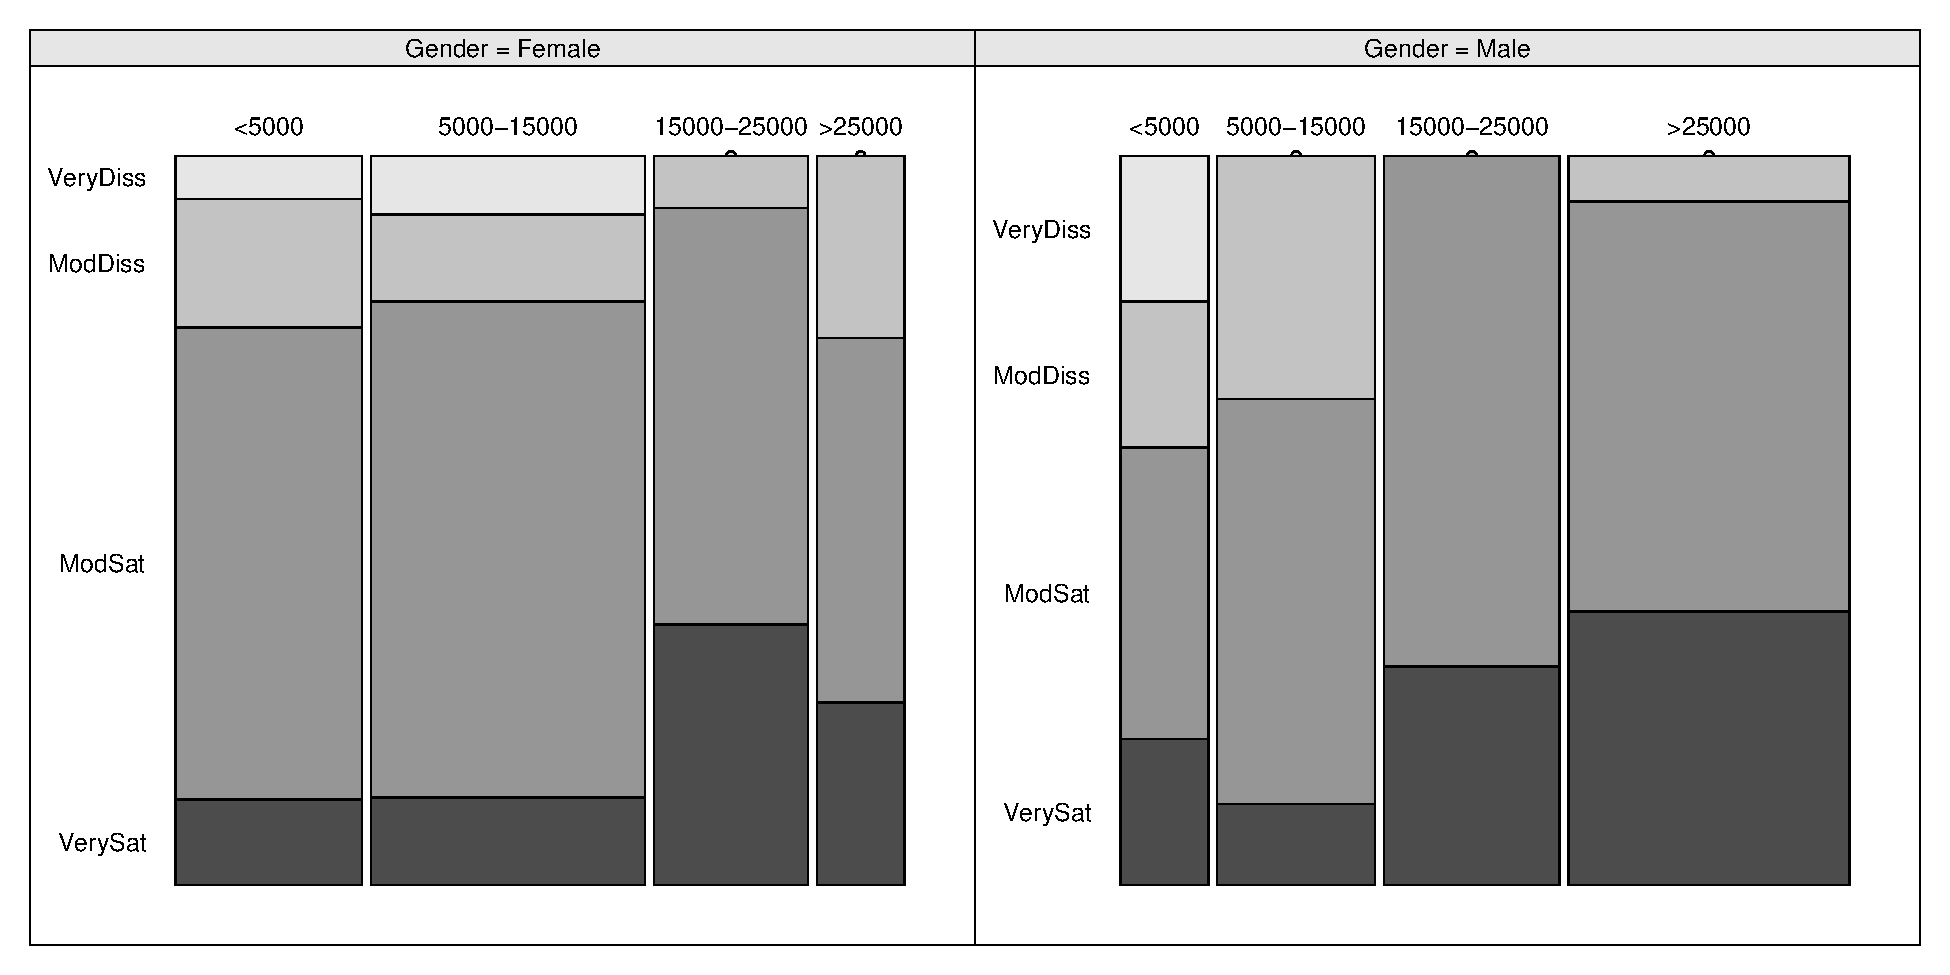
\includegraphics{coin_implementation-js-plot}
\caption{Conditional mosaic plot of job satisfaction and income given gender.
         \label{jsplot}}
\end{center}
\end{figure}
The Cochran-Mantel-Haenszel test---a classical test for testing independence
in stratified contingency tables---could be used for
assessing the independence hypothesis of income and job satisfaction (stratified by gender).
Traditionally, this test employs a $c_\text{quad}$ statistic derived from the contingency table
and a $\chi^2$ approximation of the null distribution:
\begin{Schunk}
\begin{Sinput}
R> it <- independence_test(js, teststat = "quad",
+    distribution = asymptotic())
R> it
\end{Sinput}
\begin{Soutput}
	Asymptotic General Independence Test

data:  Job.Satisfaction by
	 Income (<5000, 5000-15000, 15000-25000, >25000) 
	 stratified by Gender 
chi-squared = 10.2001, df = 9, p-value = 0.3345
\end{Soutput}
\end{Schunk}
Thus, the test does not indicate significant departure from independence.
However, ordering of the factors is not exploited by the Cochran-Mantel-Haenszel test.
As some positive correlation of the two factors would seem natural, it is worth
having a closer look at the data and the test result. The underlying linear statistic is
\begin{Schunk}
\begin{Sinput}
R> statistic(it, "linear")
\end{Sinput}
\begin{Soutput}
            VeryDiss LitSat ModSat VerySat
<5000              2      4     13       3
5000-15000         2      6     22       4
15000-25000        0      1     15       8
>25000             0      3     13       8
\end{Soutput}
\end{Schunk}
This is exactly the original contingency table
aggregated over the block factor \code{Gender}:
\begin{Schunk}
\begin{Sinput}
R> margin.table(js, 1:2)
\end{Sinput}
\begin{Soutput}
             Job.Satisfaction
Income        VeryDiss LitSat ModSat VerySat
  <5000              2      4     13       3
  5000-15000         2      6     22       4
  15000-25000        0      1     15       8
  >25000             0      3     13       8
\end{Soutput}
\end{Schunk}
Therefore, the standardized linear statistic can be interpreted similarly
to Pearson residuals for the independence hypothesis:
\begin{Schunk}
\begin{Sinput}
R> statistic(it, "standardized")
\end{Sinput}
\begin{Soutput}
              VeryDiss      LitSat     ModSat    VerySat
<5000        1.3112789  0.69201053 -0.2478705 -0.9293458
5000-15000   0.6481783  0.83462550  0.5175755 -1.6257547
15000-25000 -1.0958361 -1.50130926  0.2361231  1.4614123
>25000      -1.0377629 -0.08983052 -0.5946119  1.2031648
\end{Soutput}
\end{Schunk}
The positive diagonal and (mostly) negative off-diagonal elements convey
that higher income categories seem to be associated with higher job
satisfaction. Thus, to direct power against ordered alternatives,
a linear-by-linear association statistic \citep{agresti2002} should be used
instead of the omnibus $\chi^2$ statistic. This can be conveniently performed
within \pkg{coin}, e.g., using simple equi-distant scores and a Monte Carlo
approximation of the null distribution:
\begin{Schunk}
\begin{Sinput}
R> it <- independence_test(js, distribution = approximate(B = 10000),
+    scores = list(Job.Satisfaction = 1:4, Income = 1:4))
R> pvalue(it)
\end{Sinput}
\begin{Soutput}
[1] 0.0116
99 percent confidence interval:
 0.009024885 0.014651019 
\end{Soutput}
\end{Schunk}
Using this strategy, the null hypothesis of independence of job satisfaction
and income can be rejected in favor of a positive association of both variables.
Other choices of scores are also conceivable. Especially when there is an underlying
numeric scale, interval midpoints are often used \citep[see][for an example]{Hothorn:2006:AmStat}.

For other patterns of dependence---e.g., when only a few cells in a large table deviate
from independence---a maximum-type statistic is also useful for contingency tables.
To complete our tour of \pkg{coin} tools for categorical data, we briefly illustrate
this approach using the job satisfaction data again (even though a maximum-type statistic is
clearly not very powerful for the dependence pattern in this data set).
The maximum-type test is set up  easily:
\begin{Schunk}
\begin{Sinput}
R> independence_test(js, teststat = "max")
\end{Sinput}
\begin{Soutput}
	Asymptotic General Independence Test

data:  Job.Satisfaction by
	 Income (<5000, 5000-15000, 15000-25000, >25000) 
	 stratified by Gender 
maxT = 1.6258, p-value = 0.7214
\end{Soutput}
\end{Schunk}
with its conditional asymptotic null distribution being 
available immediately (due to the joint multivariate normal distribution
for the contingency table $\T$). Single-step adjusted $p$~values for each
cell of the contingency table corresponding to this maximum test
can be computed via
\begin{Schunk}
\begin{Sinput}
R> pvalue(independence_test(js, teststat = "max"), method = "single-step")
\end{Sinput}
\begin{Soutput}
             VeryDiss    LitSat    ModSat   VerySat
<5000       0.9010585 0.9987783 0.9999998 0.9888276
5000-15000  0.9992724 0.9948608 0.9998850 0.7215165
15000-25000 0.9660054 0.8035550 0.9999999 0.8269899
>25000      0.9761862 1.0000000 0.9996381 0.9394694
\end{Soutput}
\end{Schunk}
These $p$~values can be interpreted in a way similar to 
standardized contingency tables. The discrepancy between the
global adjusted $p$~value shown above and the minimum single-step
adjusted $p$~value is due to simulation variance. 
For more practical examples, including
applications with numeric variables, we refer to \cite{Hothorn:2006:AmStat}.



\section{Odds and ends} \label{sec:oddsandends}

\paragraph{Internal functionality.}

The core functionality, i.e., a small set of 
functions computing the linear statistic $\T$ (both for the original and
permuted data), the conditional expectation~$\mu$
and conditional covariance matrix~$\Sigma$, is coded in \proglang{C}. 
The shift and split-up algorithms \citep{axact-dist:1986,exakte-ver:1987,vdWiel2001}
for computing the exact null distribution in 2-sample problems with univariate response
as well as conditional Monte-Carlo procedures for approximating the
exact conditional null distribution are implemented in \proglang{C} as well.
(In addition,
some helper functions, e.g., the Kronecker product etc., are coded in \proglang{C}.)
The complete \proglang{C} source code and its documentation can be accessed via
\begin{Schunk}
\begin{Sinput}
R> browseURL(system.file("documentation", "html", "index.html",
+    package = "coin"))
\end{Sinput}
\end{Schunk}
The naming scheme of the \proglang{C} routines distinguishes between functions
only called at the \proglang{C} level (\code{C_}\textit{foo}) and functions which can 
be called from \proglang{R} via the \code{.Call} interface (\code{R_}\textit{foo}). 
Such functions are available for most of the internal \proglang{C} functions to enable
unit testing.


\paragraph{Quality assurance.}

The test procedures implemented in \pkg{coin} are continuously
checked against results obtained by the corresponding implementations in
\pkg{stats} (where available). In addition, the test statistics
and exact, approximate and asymptotic $p$~values for data examples
given in the \pkg{StatXact}~6 user manual \citep{StatXact6} are compared
with the results reported there. Step-down multiple adjusted $p$~values
have been checked against results reported by \code{mt.maxT()} from
package \pkg{multtest} \citep{PKG:multtest}. For details on the test
procedures we refer to the \proglang{R} transcript files in directory
`\code{tests}' of the \pkg{coin} package sources.

\paragraph{Computational details.}

The \pkg{coin} package imports packages \pkg{mvtnorm}
\citep{PKG:mvtnorm} for the evaluation of the multivariate normal
distribution and package \pkg{modeltools} \citep{PKG:modeltools} for
formula parsing.
The class structure, internal functionality, user interface and examples are
based on \pkg{coin} version 0.6-11, available
under the terms of the General Public License from \url{http://CRAN.R-project.org/}. 
\proglang{R} version 2.7.1 \citep{rcore2007}
was used for the computations, Figure~\ref{jsplot} was created using the \pkg{vcd} 
package \citep{vcd}.

\section*{Acknowledgments}
 
We would like to thank Helmut Strasser for discussions on the theoretical framework.
Henric Nilsson provided clarification and examples for the Maxwell-Stuart test and helped
identifying bugs. The work of Torsten Hothorn was supported by Deutsche Forschungsgemeinschaft (DFG) 
under grant HO 3242/1-3.

\bibliography{coin}

\newpage

\begin{appendix}

\section{Expectation and covariance} \label{app}

The conditional expectation and covariance matrix of linear statistics
$\T$ as given in Equation~\ref{linstat} in Section~\ref{sec:theory} are computed
as follows.
Let $w_{\cdot j} = \sum_{i = 1}^n I(b_i = j)w_i$ denote the sum of the weights
in block $j$ and $S_j$ the set of all permutations of the observations in block $j$. 
The conditional expectation of the transformation $h$ in block $j$ is
\begin{eqnarray*}
\E(h | S_j) = w_{\cdot j}^{-1} \sum_i I(b_i = j)w_i h(\Y_i) \in \R^q
\end{eqnarray*}
with corresponding $q \times q$ covariance matrix
\begin{eqnarray*}
\V(h | S_j) = w_{\cdot j}^{-1} \sum_i I(b_i = j)w_i \left(h(\Y_i) - \E(h | S_j)
\right) \left(h(\Y_i) - \E(h | S_j)\right)^\top.
\end{eqnarray*}
This is the basis for computing the conditional expectation and covariance of the linear statistic
$\T_j$ in block $j$:
\begin{eqnarray*}
\mu_j & = & \E(\T_j | S_j) = \vec \left( \left( \sum_{i = 1}^n I(b_i = j)w_i g(\X_i) \right) \E(h | S_j)^\top
\right)
\end{eqnarray*}
and
\begin{eqnarray*}
\Sigma_j & = & \V(\T_j | S_j) \nonumber \\
& = &
    \frac{w_{\cdot j}}{w_{\cdot j} - 1}  \V(h | S_j) \otimes
        \left(\sum_i I(b_i = j) w_i  \left( g(\X_i) \otimes g(\X_i)^\top\right) \right)
\label{expectcovar}
\\
& - & \frac{1}{w_{\cdot j} - 1}  \V(h | S_j)  \otimes \left(
        \sum_i I(b_i = j) w_i g(\X_i) \right)
\otimes \left( \sum_i I(b_i = j) w_i g(\X_i)\right)^\top
\nonumber
\end{eqnarray*}
where $\otimes$ is the Kronecker product. The conditional
expectation and covariance of $\T$, aggregated over all $k$ blocks, are
then given by
\begin{eqnarray*}
\E(\T | S_j) & = & \mu  \; = \; \sum_{j = 1}^k \mu_j  \; = \; \sum_{j = 1}^k \E(\T_j | S_j), \\
\V(\T | S_j) & = & \Sigma \; = \; \sum_{j = 1}^k \Sigma_j \; = \; \sum_{j = 1}^k \V(\T_j | S_j).
\end{eqnarray*}

\end{appendix}

\end{document}
